\chapter{Qualitative Description Of The Simulation}
Computers have been used for numerical studies since their invention. Especially in the field of nonlinear dynamics and complex systems they are the only useful tool to analyze certain systems because their chaotic behavior can not be easily predicted using analytical studies. Different styles of simulations haven been developed throughout the days. For the simulation of the disease spread in the case of BVD we decided to use an agent and event based model with compared with a stochastically motivated approach to calculating the infection probability and other important dynamics. The statistical data which is defining the systems data has been provided by \citep{personalCom} and further explored by \footnote{Zitat auf Inias Masterarbeit}. This chapter will explain the details of the setup system.
\section{Event based simulation}
Most numerical studies work with quasi continuous integrators. By changing the system state in small time steps $dt$ the system can be approximated. Another approach has been chosen for this simulation. Some integrators adapt the time steps $dt$ so that only noticeable changes in system states can be noticed. The event based simulation uses a very similar approach. The system calculates the time of the next event and skips the time interval till the next event. One event can trigger a series of other events that will be scheduled. 
\section{Cows (Agents)}
The simulation which has been developed for this study is an agent based simulation. The life cycle of every single cow is simulated and tracked. Cows are the smallest entity of the simulation. Their state is made up of different variables. A calve will only become a new entity of type Cow at the time of birth. The most important variables are 
\begin{itemize}
\item date of birth (to calculate the age),
\item a list of calves and their birth dates (to calculate the intermediate calving time),
\item health state in regard of their BVD status,
\item reproductional status (is there a calf and what is it's status?),
\item sex,
\item the remaining number of calves and
\item status of the last test.
\end{itemize}

\section{Farms}
Farms build up the different nodes of the system. Each farm can be made up of an arbitrary number of herds and a farm manager. The different implemented types will show a differences in their behaviour mainly defined by their farm manager.
\subsection{Farm Types}
So far 4 types of farms have been implemented which are listed below. The influence of fattening farms has been neglected so far because we did not have any data on which farms are fattening farms and because fattening farms should not have a big influence on the disease spread, since they use male cows which can not create new PIs.
\paragraph{Simple One Herd Farm}
The simple one herd farm (as it's name suggests) has a single herd. It will try to hold it's herd size within the boundaries given via the ini file. Furthermore it will try to rejuvinate it's population by selling a certain amount of it's population also defined by the ini file of a given time frame and then buying the same amount of cows from other farms. The default value for the rejuvination has been set to $27.9\,\%$ per year according to the yearly replacement rate given by Gethmann
\paragraph{Slaughterhouse}
The slaughterhouses action will be defined by the ini file too. Either it buys all cows which have not been bought at the end of a market period or it will buy a given amount of cows per market period. One system can have an arbitrary amount of slaughterhouses.
\paragraph{Small One Herd Farm}
The small one herd farm shows the exact same behaviour as the simple one herd farm except for the rejuvination. The threshold in size between the simple and the small one herd farm can bet set via the ini file. 
\paragraph{Cow Source Farm}
The cow source farm will create new cows to put them into the system in order to keep the amount of cows in the system constant. They just sell pregnant cows. If the slaughterhouse buys a fixed amount of cows, the cow well farm will also offer a fixed amount of cows. If the slaughterhouse just works as sink for all cows which have not been sold, the cow well farm will be asked to create enough cows to satisfy the demand of all farms that hasn't been satisfied yet.
\subsection{Farm Manager}\label{chap:farmManager}
The farm manager describes the behavior of the farm. So far it only calculates, which cows should be sold and how many cows of which type should be bought. Most farmers in reality would try to only buy pregnant cows, because they already survived their youth and will start giving milk right after the birth of their calf and the calf can be sold or raised right away\footnote{This hypothesis has only been supported by personal conversations and has not yet been supported by data from HI Tier.}.
\subsection{Herds}
A herd is a group of cows. The next infection event will calculated on a farm level calculating the transition rate following \citep{VIE04} (equation \ref{eq:vie04}). Other than that the herd only keeps track of the different compartments and the demography of it's members.
\section{Disease Spread}
BVD spreads from one farm to another within the body of an infected cow. Therefore only the disease dynamics within a farm need to be simulated with their own code. The description of the trading system is placed in section \ref{chap:tradeDesc}. As mentioned above, the simulation takes a stochastic approach to modeling the disease dynamics. The time of the next infection in a farm is calculated with the following: \\
\begin{enumerate}
\item The transition probabilities $\lambda_\text{SI}^k$ for every single herd $k$ are calculated following equation \ref{eq:vie04start}.
\item Then the inter herd transmission coefficients $\beta^{kl}_\text{PI}$ from herd $k$ to herd $l$ are used to calculate the full transition rate:
\begin{equation}
\lambda_\text{SI}^k = \lambda_\text{SI} + \sum_{l \neq k} \beta^{lk}_\text{PI} P^l
\end{equation}
given in \citep{VIE04}. The probability $\beta_\text{SI} \in [0.1,0.3] $ is relatively low compared to $\beta_\text{PI} \geq 0.99$, which is why it can be neglected for the inter herd transmission.
\item The total infection rate for all herds is then calculated multiplying by $S^k$: $p^{(k)} = S^k \lambda_\text{SI}^k $. Note that if we would handle herds of a farm as a network of herds with a Adjacency matrix $A$ with entries $a_{ij}$, we would be able to write $\beta_\text{PI}^{kl}= \beta_\text{PI} a_{lk}$ because we use the convention of an entry $a_{ij}$ corresponding to a link between node $j$ and node $i$.
\item The time $t^k$ for the next infection in this herd is calculated using\\ {\tt gsl\_ran\_exponential($1/p^{(k)}$)} from the gnu scientific library.
\item The shortest time is chosen to schedule the next infection event, if it is not bigger then the execution time of any already scheduled infection event.
\end{enumerate}
This process is repeated every time the infection rate changes. This happens when any of the cows changes it's health state, a new cow is born or a cow dies or a trade occurs. 
\section{Trading}\label{chap:tradeDesc}
The trading behavior of the whole system is defined by multiple fractions. It all starts with the farm managers and is then organized by the market. The basic scheme is shown in figure \ref{fig:tradingScheme}.
\begin{figure}[htbp]
\centering
\noindent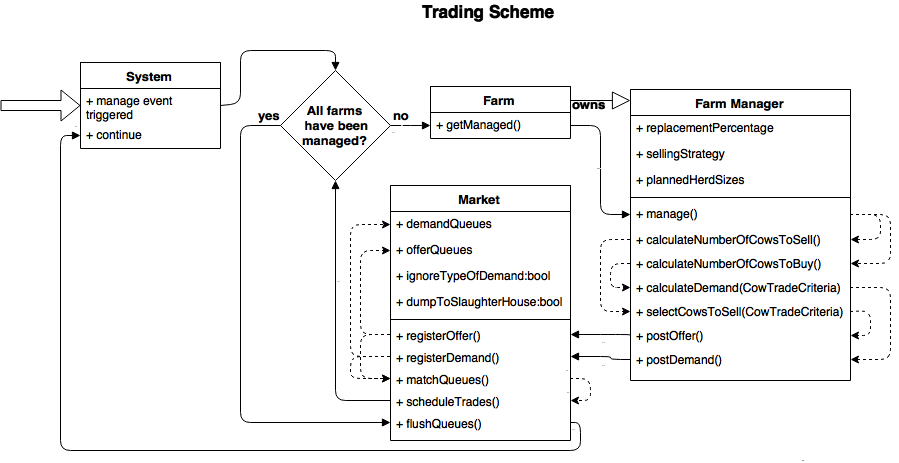
\includegraphics[width=0.8\linewidth,height=\textheight,
keepaspectratio]{MarketFlow.png} 
\caption[Trading Scheme]{The picture shows the basic scheme of the whole trading system. All in all the system is a little more complex, but this diagram gives a good idea on the process. The upper section of an object's box contains it's relevant member variables whereas the lower part contains the most important functions. Note that not all function names resemble the function names in the code by a hundred percent.}
\label{fig:tradingScheme}
\end{figure}
\subsection{Farm Manager}
The trading is processed once every trading period $T$ which can be set using the ini file. It is triggered by the global {\tt MANAGE} event. All farm managers will be asked to register cows at the market using the market's {\tt register\_offer} method and ask for new cows using the market's {\tt register\_demand} method. They can specify the amount of cows they'd like to receive for one of the following so called {\tt Cow\_Trade\_Criteria} shown in \ref{tab:cowTradeCrit}, but the market can be set to ignore this preference. 

\begin{table}[htb]
    \begin{center}
    \begin{tabular}{|ccc|}\hline
        \rowcolor{dunkelgrau} Cow\_Trade\_Criterium  & sex [m/f] & age [days] or other criterium \\\hline
                              CALF  & f& $\leq {\tt bvd\_const::age\_threshold\_calf}$\\\hline
\rowcolor{hellgrau}           HEIFER\_PRE\_BREEDING  & f& $\leq 527$\footnotemark \\\hline
                              HEIFER\_RDY\_BREEDING  & f& every other age \\\hline
\rowcolor{hellgrau}           INFERTILE  & f& female, infertile cow\footnotemark \\\hline
                              PREGNANT  & f& is pregnant\\\hline
\rowcolor{hellgrau}           DAIRY\_COW  & f& has had a calve\\\hline 
                              OLD\_COW & f& $> 1488 $\\ \hline
\rowcolor{hellgrau}            MALE\_CALF &   m & $\leq {\tt bvd_const::age\_threshold\_calf}$   \\\hline
                               YOUNG\_BULL & m  &  $\leq 186$  \\\hline 
\rowcolor{hellgrau}           OLD\_BULL   &  m  & every other bull   \\\hline           
\end{tabular}
\caption[Explanation of Cow Trade Criteria]{Different cow trade criteria as they are defined in code. The {\tt bvd\_const::age\_threshold\_calf} is set in {\tt Model\_Constants.h}. At the time of writing this, it is set to $ 180 \, \text{days} $.}
\label{tab:cowTradeCrit} 
\end{center}
\end{table}
\footnotetext{Until now this values has been fixed, but it could be changed in the future.}
\footnotetext{This is not used yet, since no cows become infertile.}
For all experiments in this thesis it has been decided to set the preference of all farms to buy {\tt PREGNANT} cows only according to the hypothesis given in section \ref{chap:farmManager}. 
Currently two different ways of deciding which cows to offer at the market are implemented. After the farm manager has calculated how many cows it wants to sell, it has two decide, how to distribute this number between the different {\tt Cow\_Trade\_Criteria}. For this it has a list of lists of criteria. It will work through the outer list until it satisfied it's needs for cows to sell. It will split up the number of cows it needs evenly on all criteria of the inner list. Currently two different combinations have been implemented. The first selling strategy {\tt evenlyDistributed} has only one inner list containing all criteria so that it will split up the number of cows to sell evenly on them. The other strategy {\tt OldCowsFirst} contains the following lists
\begin{itemize}
\item MALE\_CALF, YOUNG\_BULL, OLD\_BULL, INFERTILE
\item OLD\_COW
\item HEIFER\_PRE\_BREEDING  
\item HEIFER\_RDY\_BREEDING
\item CALF
\item PREGNANT, DAIRY\_COW .
\end{itemize}

\subsection{Market}\label{chap:market}
The market receives the various demands and offers and processes it. Depending on it's configuration it will behave differently.
\paragraph{Registering Offers And Demands}
First the cows and demands get stored in containers, which are queues in the current implementation. If the market is set to respect the demand of the different farms, it will create a queue for each {\tt Cow\_Trade\_Criteria}, else it will just create one queue for all offers and one queue for all demands. When a demand or offer has been placed, it will be put at the end of the corresponding queue. After that the market will try to match the offers and demands in the queue (see figure \ref{fig:tradingScheme}). If the slaughterhouse is set to work in \glqq demand\grqq mode, both the slaughterhouse and the cow well farm will register offers and demands according to the settings in the ini file. If the mode is set to \glqq dump\grqq, they will only get important during the phase of flushing the queues.

\paragraph{Flushing The Queues}
After all farms have posted all their offers and demands and all of them have been matched, the queues get flushed. If the slaughterhouse does not work as a sink, it will simply empty the queues, else the cows from all offers will be dumped to it and all demands will be satisfied by cows from the cow well farm (compare \ref{chap:farmManager}). When the market tries to schedule a trade, it will run different filters on it first. By now the filters only make sure that the source farm does not trade with a slaughterhouse and that a farm does not trade with itself. If a trade is rejected by the filters, the cow will be pushed on a buffer queue (to avoid trying it more then once). After all possible matches have been processed, the cows from the bufferQueue will be pushed back to the corresponding queue in the market.

\section{Containment Strategies}
All containment strategies are implemented system wide. They are turned on and off by special events which can be set using the ini file. 
\subsection{Eartag Testing}
If the testing is enabled, the first test is executed right after birth. If it is tested positive, it will be retested after a period that can be set using the ini file, assuming the worst case that farmers will rather retest than culling more calves then necessary. In case the quarantine should be applied, it will be applied right after a first positive test. The time of the quarantine can be set using the ini file too. 
\subsection{Vaccination}
If vaccination is applied on animals, the first vaccination will be scheduled after ${\tt bvd\_const::firstVaccAge}= 180\,\text{days}$. After that the vaccination is either applied when it ends or at least $n$ days before the next insemination. This value can be set using the ini file. The standard value for this is $n=42\,\text{days}$ according to the information given by \citep{personalCom}. For the time the cow is vaccinated, it will be put in the group of immune animals. According to Gethmann there is a little chance that cows could get infected by the vaccination, but this would not enable them to infect others or have an impact on the foetus. Since this would actually better, because the cow would get be immune for the rest of it's life, ignoring this case, like it is done by now, will have no positive impact on the system.
\subsection{YCW}
The farm manager is asked every half a year or every year to test cows as they are specified in the description above. For now only the scheme of Thuringia is implemented. 